\documentclass[11pt]{article}  
\usepackage[margin=1in]{geometry}
\parindent=0in
\parskip=8pt
\usepackage{fancyhdr,amssymb,amsmath, graphicx, listings,float,subfig,enumerate,epstopdf,color,multirow,setspace,bm,textcomp}
\usepackage[usenames,dvipsnames]{xcolor}
\usepackage{hyperref}
\usepackage{graphicx}
\usepackage{tikz}
\graphicspath{{./Images}}

\pagestyle{fancy}


\begin{document} 

\lhead{Assignment \# 1}
\chead{Robert Denim Horton}
\rhead{\today}

\begin{center}\begin{Large}
CS 4720/5720 Design and Analysis of Algorithms
Homework \#1
Student: (Robert Denim Horton)
\end{Large}
\end{center}

\section*{Answers to homework problems:}

\textcolor{gray}{
% Chapter 2 : Question 1
\begin{enumerate}
	\item \quad \\
	% Question 1 : Part A
	\begin{enumerate}[(a)]
		\item  Given the formal definition of a pivotal node, a node can be difeind as such when the node of intrest exsits along every shortest possible path in a given pair of nodes.  For example, given a graph with the set of nodes $S_0$ with defined nodes $\{A, \ B, \ C, \ D, E\}$.  The graph could be represented as;\\
		\begin{center}
			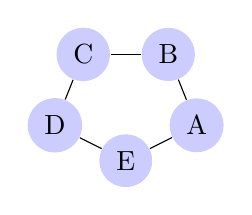
\begin{tikzpicture}[scale=0.9, auto=center, every node/.style={circle,fill=blue!20}] 
				\node(A) at (1, -0.5) {A}; 
				\node(B) at (0.6, 0.5) {B};
				\node(C) at (-0.6, 0.5) {C}; 
				\node(D) at (-1,-0.5) {D}; 
				\node(E) at (0,-1) {E}; 
				\draw(A) -- (B);
				\draw(B) -- (C);
				\draw(C) -- (D);
				\draw(D) -- (E);
				\draw(E) -- (A);
		\end{tikzpicture}
	\end{center}
As we can see in this diagram all the nodes are pivotal nodes.   Starting with node pivotal node $A$, its only pivotal node pair is $E$ and $B$, for node $B$its only pivotal node pair is $C$ and $A$, for node $C$ its only pivotal node pair is $B$ and $D$, its only pivotal node pair is $C$ and $E$, and lastly for node $E$its only pivotal node pair is $D$ and $A$.  Here we can see that every node that exsits has atleast one pair of nodes that also exists in the graph.\\
% Question 1 : Part B
	\item For a pivotal node to have two different pairs of pviotal nodes, we can again define a node with two different pairs of pivotal nodes as a node that is along the fatest path for tow nodes but with the added implication that this node is along one other pair of pivotal nodes. With the same set, $S_0$, from part a we can consruct a graph to be represnted as, 
	\begin{center}
		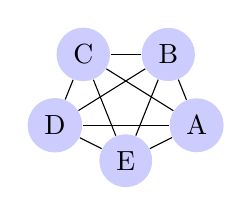
\begin{tikzpicture}[scale=0.9, auto=center, every node/.style={circle,fill=blue!20}] 
			\node(A) at (1, -0.5) {A}; 
			\node(B) at (0.6, 0.5) {B};
			\node(C) at (-0.6, 0.5) {C}; 
			\node(D) at (-1,-0.5) {D}; 
			\node(E) at (0,-1) {E}; 
			\draw(A) -- (B);
			\draw(A) -- (C);
			\draw(B) -- (C);
			\draw(B) -- (D);
			\draw(C) -- (D);
			\draw(C) -- (E);
			\draw(D) -- (E);
			\draw(D) -- (A);
			\draw(E) -- (A);
			\draw(E) -- (B);
		\end{tikzpicture}.
	\end{center}
We can see that for every node in the graph, it has atleast two different pairs of pivotal nodes.  Node $A$ has it's first pivotal nodes as $E$ and $B$ and second pair of pivotal nodes $C$ and $D$,  node $B$ has it's first set of pivotal nodes $C$ and $A$ and second pair of pivotal nodes $E$ and $D$, node $C$ has it's first set of pivotal nodes $E$ and $A$ and it's second set of pivotal nodes $B$ and $D$, node $D$ has it's first set of pivotal nodes $B$ and $A$ and second pair of pivotal nodes $C$ and $E$, node $D$ has it's first pair of pivotal nodes $B$ and $A$ and it's second set of pivotal nodes $E$ and $C$, and lastly node $E$ has it's first pair of pivotal nodes $C$ and $B$ and it's second set of pivotal nodes $A$ and $D$.\\
% Question 1 : Part C
	\item  For a graph comprised of atleast 4 nodes where a single node is pivotla for any pair of nodes that comprise a pivotal pair.  So with a different set, $S_1$, of nodes \{$A$, $B$, $C$, $D$, $X$\} we can use a graph to represnt a graph where node $X$ is the node of intrest, \\  
	\begin{center}
		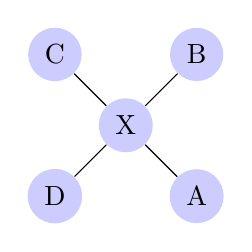
\begin{tikzpicture}[scale=0.9, auto=center, every node/.style={circle,fill=blue!20}] 
			\node(A) at (1, -1) {A}; 
			\node(B) at (1, 1) {B};
			\node(C) at (-1, 1) {C}; 
			\node(D) at (-1,-1) {D}; 
			\node(X) at (0,0) {X}; 
			\draw(A) -- (X);
			\draw(B) -- (X);
			\draw(C) -- (X);
			\draw(D) -- (X);
		\end{tikzpicture}.
	\end{center}
Here we that node $X$ has a pivotla pair with every node that is not $X$ in the graph.  So node $X$ has pivotal pairs $A$ and $C$, pivotal pair $B$ and $D$, pivotal pair $A$ and $B$, pivotal pair $C$ and $B$, pivotal pair $D$ and $A$, and pivotal pair $C$ and $D$. So six possible pairs in total.\\
	\end{enumerate}
\end{enumerate}
}
% Chapter 2 : Question 2
\textcolor{gray}{
\begin{enumerate}
\setcounter{enumi}{1}
	\item \quad \\
	\begin{enumerate}[(a)]
		\item Give an example (together with an explanation) of a graph in which more than half of all nodes are gatekeepers.
		\item Give an example (together with an explanation) of a graph in which there are no gatekeepers, but in which every node is a local gatekeeper
	\end{enumerate}
\end{enumerate}
}

% Chapter 2 : Question 3
\textcolor{gray}{
\begin{enumerate}
\setcounter{enumi}{2}
	\item \quad \\
	\begin{enumerate}[(a)]
		\item Describe an example of a graph where the diameter is more than three times as large as the average distance.\\
		\item Describe how you could extend your construction to produce graphs in which the diameter exceeds the average distance by as large a factor as you’d like. (That is, for every number c, can you produce a graph in which the diameter is more than c times as large as the average distance?)\\
	\end{enumerate}
\end{enumerate}
}
\end{document}
